
\documentclass{beamer}
\usepackage{graphicx}
\usepackage[super]{nth}
\usetheme{Malmoe}
\newcommand{\ts}{\textsuperscript}

\makeatletter
    \newenvironment{withoutheadline}{
        \setbeamertemplate{headline}[default]
        \def\beamer@entrycode{\vspace*{-\headheight}}
    }{}
\makeatother

\addtobeamertemplate{navigation symbols}{}{%
    \usebeamerfont{footline}%
    \usebeamercolor[fg]{footline}%
    \hspace{1em}%
    \insertframenumber/\inserttotalframenumber
}

%%%%%%%%%%FIRST SLIDE%%%%%%%%%%

\setbeamercolor*{title}{use=structure,fg=white,bg=structure.fg}
\setbeamertemplate{title page}[default][colsep=-4bp,rounded=true,shadow=true]
\title[Collision Prevention in Distributed 6TiSCH Networks]{Collision Prevention \\in Distributed 6TiSCH Networks}

\author{ Ali Jawad Fahs\\}


\institute[Universities of Somewhere and Elsewhere] % (optional, but mostly needed)
{Universit\'e Grenoble Alpes (UGA) - UFR IM\textsuperscript{2}AG \\

Laboratoire d'Informatique de Grenoble (LIG), Team Drakkar \\
VERIMAG,Synchrone\\
Supervised by : Olivier Alphand, Franck Rousseau \\
 Karine Altisen, St\'ephane Devismes 
 }

\date{Master thesis, \nth{21} of June,2017}


\subject{Wireless Sensor Networks}
%%%%%%%%%%%%%%%%%%%%%%%% OUTLINE%%%%%%%%%%%%
\AtBeginSubsection[]
{ \begin{withoutheadline}
  \begin{frame}<beamer>{Outline}
    \tableofcontents[currentsection,currentsubsection]
  \end{frame}
  \end{withoutheadline}
}

%%%%%%%%%%%%%%%%%%%% SLIDES %%%%%%%%%%%%%%%%
\begin{document}
\begin{withoutheadline}
\begin{frame}
  \titlepage

\begin{itemize}
\item[]
\begin{center}

\includegraphics[width=0.2\linewidth]{logo_im2ag_h122.jpg} \hskip 1em

\includegraphics[width=0.25\linewidth]{logoINP.png}  \hskip 1em

\includegraphics[width=0.21\linewidth]{LIG_test.png}  \hskip 1em

\includegraphics[width=0.22\linewidth]{verimag.jpg}
\end{center}
\end{itemize}


\end{frame}
\end{withoutheadline}

\begin{withoutheadline}
    \begin{frame}{Outline} % and our simple frame
        \tableofcontents
    \end{frame}
\end{withoutheadline}

%%%%%%%%%%%%%%%%%%%%%%%%%%%%%INTRO%%%%%%%%%%
\section{Introduction}

\subsection{General intoduction}
\begin{withoutheadline}
\begin{frame}{General introduction}{IoT \& Wireless Sensor Networks}
\setbeamercolor{block title}{bg=blue!30,fg=black}
\setbeamercolor{block body}{bg=blue!10,fg=black}
\setbeamertemplate{blocks}[rounded][shadow=false]
 \begin{block}{IoT}
    \begin{itemize}
    \item Historically networks were a connection of high performance expensive computers.
    \item<2-> Nowadays network is a connection of entities with limited processing capabilities called Things. 
    \item<3->  led us to the idea of {\em Internet of Things (IoT)}
    \end{itemize}
  \end{block} 
  
\only<4-6>  {
\begin{block}{Wireless Sensor Networks}
    \begin{itemize}
    \item<4-> A source of communication between the IoT nodes.
    \item<5-> Main contributions are : low power, low cost.
    \item<6->  IEEE802.15.4 one of the main standard for those Networks
    \end{itemize}
    \end{block}}

  
  
\end{frame}
\end{withoutheadline}




\begin{withoutheadline}
\begin{frame}{General intoduction}{IEEE802.15.4}

\setbeamercolor{block title}{bg=blue!30,fg=black}
\setbeamercolor{block body}{bg=blue!10,fg=black}
\setbeamertemplate{blocks}[rounded][shadow=false]


\begin{minipage}[t]{0.48\linewidth}

\begin{block}{IEEE802.15.4}
    \begin{itemize}
    \item The low layers of the network (i.e., PHY and MAC) 
    \item<2-> The Physical Layer and Medium Access Control Layer.
    
    \item<3-> Uses RPL to set-up A DODAG.
    \item<4-> A converge cast towards a sink. 
    
    \end{itemize}
    \end{block}
\end{minipage}\hfill
\begin{minipage}[t]{0.48\linewidth}
\centering
 \begin{figure}[p]

 \only<3>{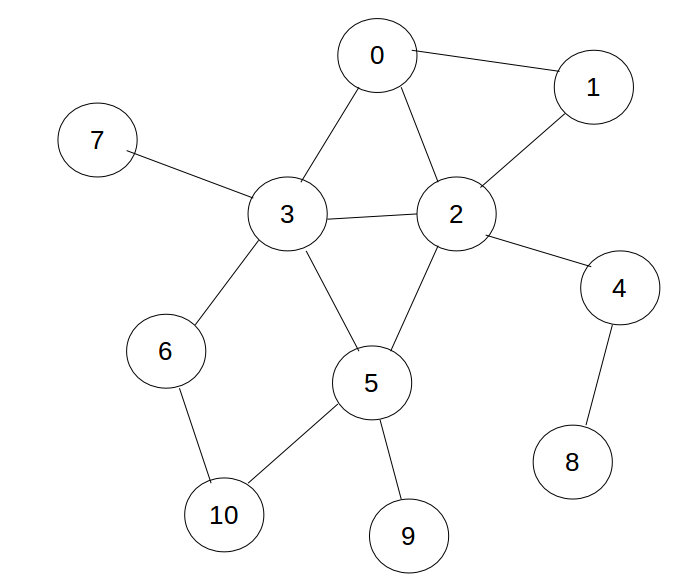
\includegraphics[width=\linewidth]{rpl1.png}}
  \only<4>{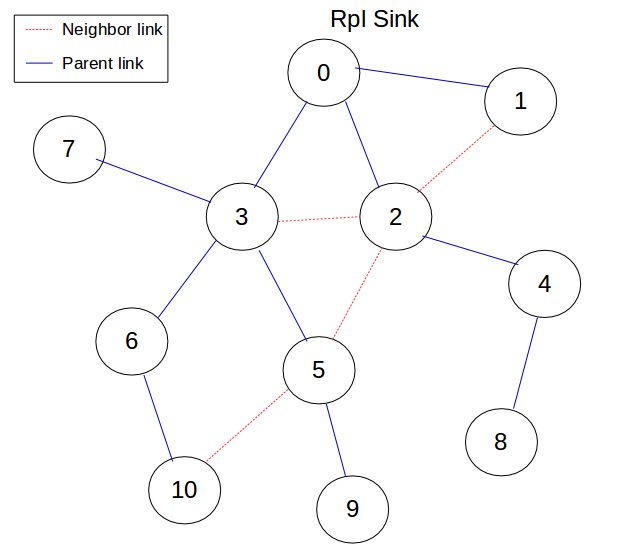
\includegraphics[width=\linewidth]{rpl2.png}}
  \only<5>{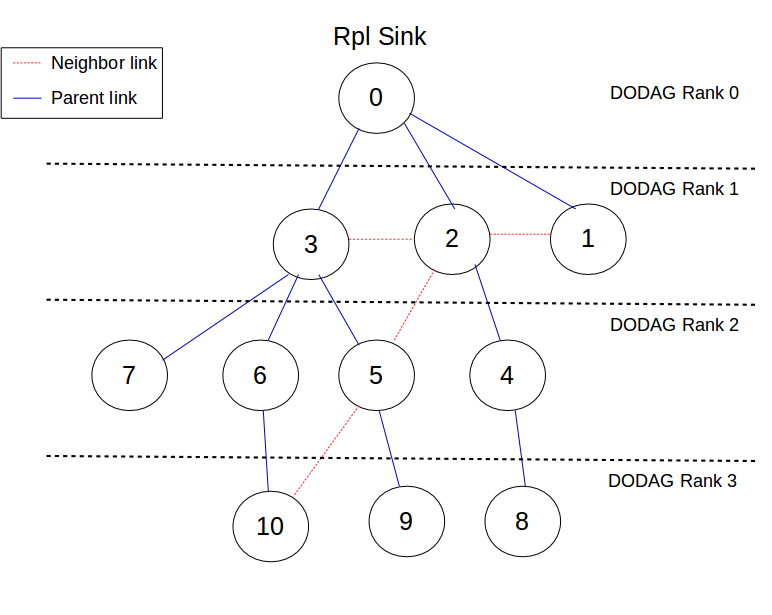
\includegraphics[width=\linewidth]{rpl3.png}}
  
  
\end{figure}
\end{minipage}

   
    
    

\end{frame}
\end{withoutheadline}




\begin{withoutheadline}
\begin{frame}{General intoduction}{IEEE802.15.4}

\setbeamercolor{block title}{bg=blue!30,fg=black}
\setbeamercolor{block body}{bg=blue!10,fg=black}
\setbeamertemplate{blocks}[rounded][shadow=false]




\begin{block}{IEEE802.15.4e TSCH}
    \begin{itemize}
    \item Extension of the Medium Access Control (MAC) Layer.
    \item<2-> Time-slotted Channel Hopping (TSCH) is based on time frequency multiplexing. 
    \item<3-> Two types of cells: dedicated and shared.
    \item<4-> Managed in centralized or distributed way. 
    
    \end{itemize}
    \end{block}

\centering
\begin{figure}[p]

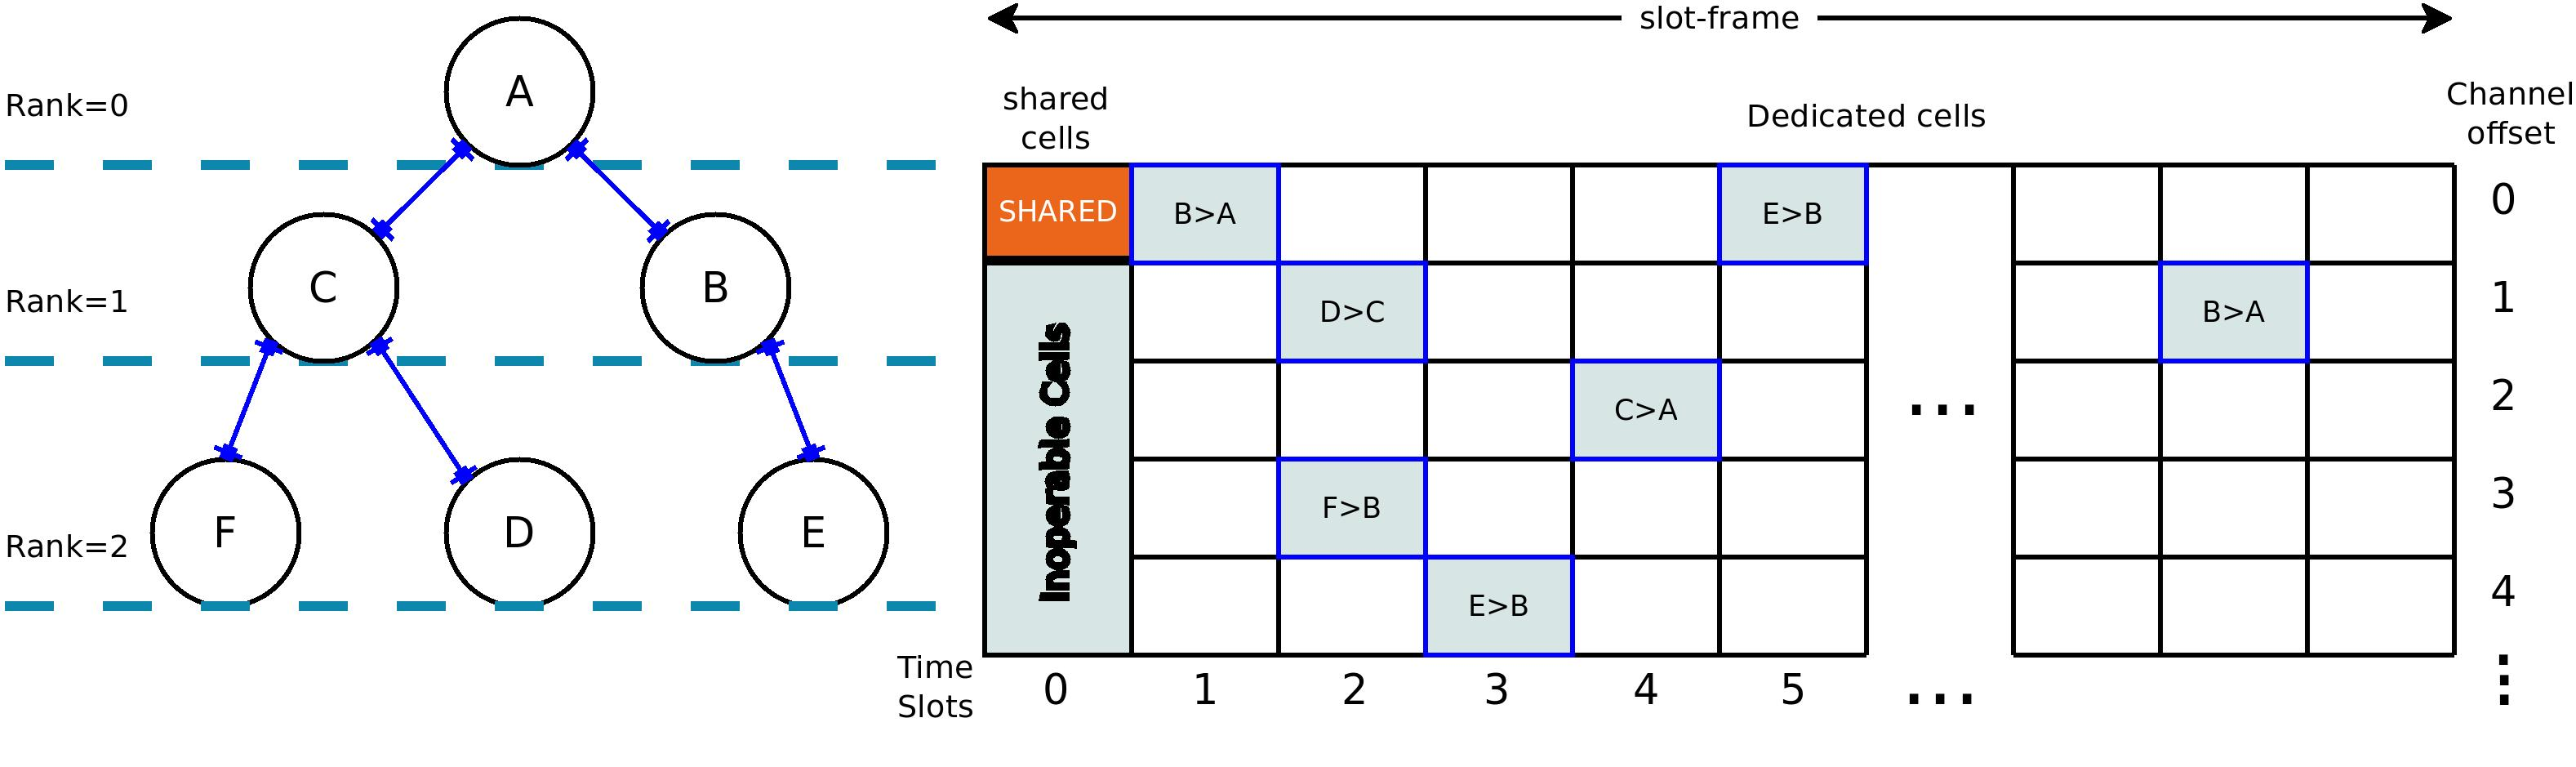
\includegraphics[width=\linewidth]{TSCh.jpeg}
\end{figure}


\end{frame}
\end{withoutheadline}

\begin{withoutheadline}
\begin{frame}{General intoduction}{Collision in the Dedicated Cells}

\setbeamercolor{block title}{bg=blue!30,fg=black}
\setbeamercolor{block body}{bg=blue!10,fg=black}
\setbeamertemplate{blocks}[rounded][shadow=false]

\begin{block}{IEEE802.15.4e TSCH}
    \begin{itemize}
    \item  Collision free dedicated cells.
    \item<2-> Collisions in distributed approach .
    \item<3-> Lack of central entity.
    \item<4-> Collision are very expensive in Wireless sensor Networks.
      
    \end{itemize}
    \end{block}
  \centering
\begin{figure}[p]

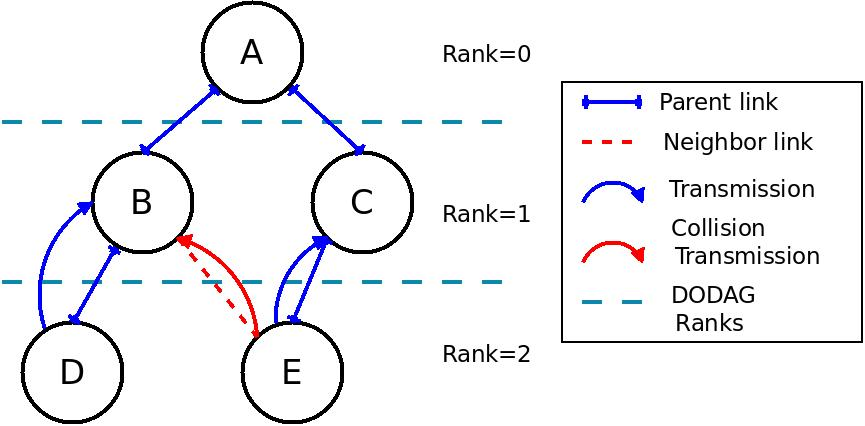
\includegraphics[width=0.7\linewidth]{col1.png}
\end{figure}  
    




\end{frame}
\end{withoutheadline}


\subsection{Project Objectives}
\begin{withoutheadline}
\begin{frame}{Project Objectives}
  \begin{itemize}
  \item {Reducing the collisions in TSCH dedicated cells.}
  \item<2-> {Modifying the Cell reserving process without introducing new overhead on the network}
  \item<3-> {Creating a flexible mechanism, compatible with all scheduling functions }

  
  \end{itemize}
\end{frame}
\end{withoutheadline}


%%%%%%%%%%%%%%%%%%%%%%%BACKGROUD%%%%%%%%%%%%%%


\section{Background}
\subsection{IEEE802.15.4e \& 6top}
\begin{withoutheadline}
\begin{frame}{IEEE802.15.4e and 6top}
\setbeamercolor{block title}{bg=blue!30,fg=black}
\setbeamercolor{block body}{bg=blue!10,fg=black}
\setbeamertemplate{blocks}[rounded][shadow=false]




\begin{block}{6TiSCH}
    \begin{itemize}
    \item The standard have defined TSCH schedule but the control of this schedule  was left for other protocols for flexibility and optimization.
    \item<2-> 6TiSCH purpose is the Integration of IPv6 and TSCH. 
    \item<3-> 6TiSCH operation (6top) is a sublayer of 6TiSCH.
    \item<4-> 6top contains the scheduling function. 
    \item<5> 6top is responsible for the cell addition and deletion. 
    
    \end{itemize}
    \end{block}
\end{frame}
\end{withoutheadline}

\begin{withoutheadline}
\begin{frame}{IEEE802.15.4e and 6top}
\setbeamercolor{block title}{bg=blue!30,fg=black}
\setbeamercolor{block body}{bg=blue!10,fg=black}
\setbeamertemplate{blocks}[rounded][shadow=false]


\begin{minipage}[t]{0.48\linewidth}

\begin{block}{6top}

    \begin{itemize}
    \item Orchestrates all communications using the TSCH schedule.
    \item<2-> Allows the nodes to request for new TSCH cells.
    \item<3-> 6top enables the distributed scheduling in 6TiSCH network.
    \end{itemize}
    \end{block}

\end{minipage}\hfill
\begin{minipage}[t]{0.48\linewidth}
\centering
\begin{figure}[p]

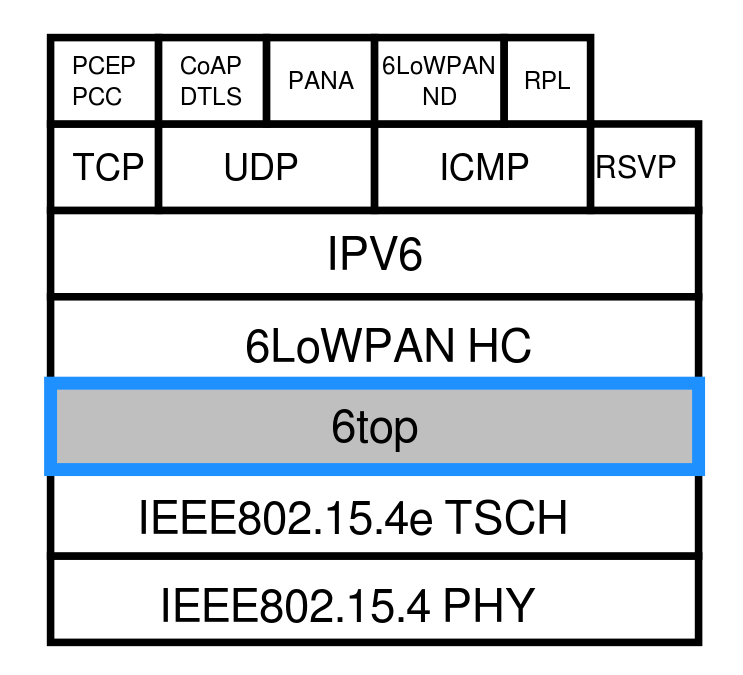
\includegraphics[width=\linewidth]{layers.png}
\end{figure}
\end{minipage}


\end{frame}
\end{withoutheadline}

\begin{withoutheadline}
\begin{frame}{IEEE802.15.4e and 6top}
\setbeamercolor{block title}{bg=blue!30,fg=black}
\setbeamercolor{block body}{bg=blue!10,fg=black}
\setbeamertemplate{blocks}[rounded][shadow=false]




\begin{block}{IEEE802.15.4e \& 6top}
    \begin{itemize}
    \item 6top transactions: negotiation to Add/Delete/Relocate cells. 
    \item<2-> Two types: 2-step and 3-step.
    \item<3-> The transaction is done in the shared slot. 
    \item<4-> The transaction will be received by the neighbor nodes by dropped due too MAC filtering of the messages. 
    
    \end{itemize}
    \end{block}
    \centering
\begin{figure}[p]

\item<2-> 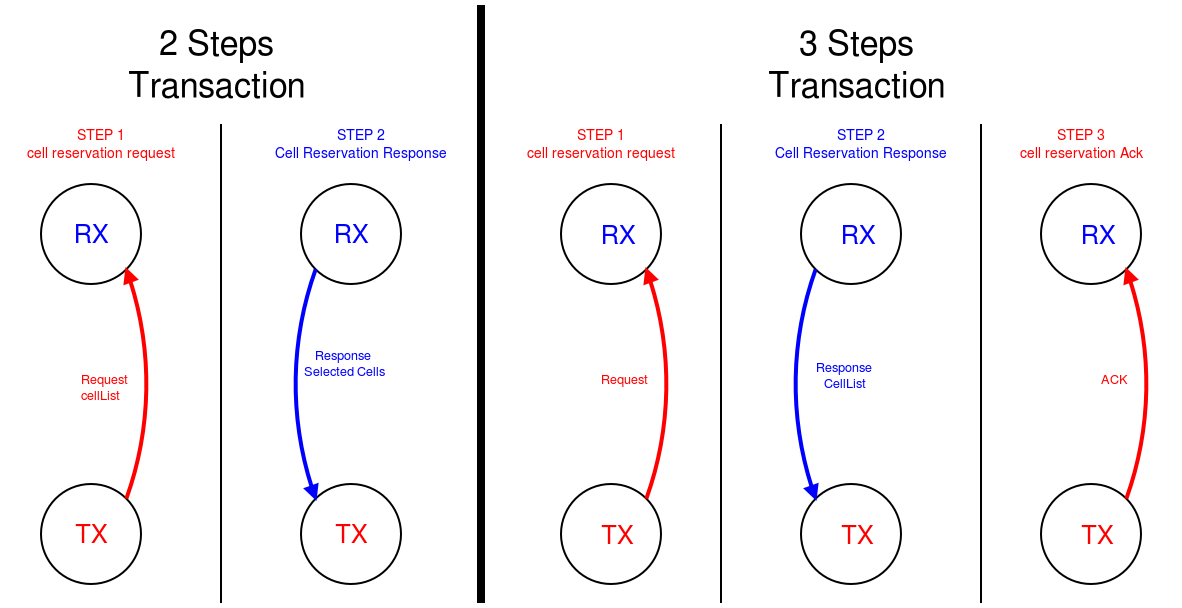
\includegraphics[width=0.6\linewidth]{2,3steps.png}
\end{figure}

\end{frame}
\end{withoutheadline}





\subsection{Collisions in Dedicated cells}


  \begin{withoutheadline}
\begin{frame}{6top and Collisions}

\setbeamercolor{block title}{bg=blue!30,fg=black}
\setbeamercolor{block body}{bg=blue!10,fg=black}
\setbeamertemplate{blocks}[rounded][shadow=false]


\begin{block}{6top}

    \begin{itemize}
    \item Nodes have no information about the neighbors.
    \item<2-> Scheduling function cell selection does not consider the neighbor's cells. 
    \item<3-> If another neighbor node is using the same cell a collision will occur. 
    \item<4-> Collisions are expensive.
    \end{itemize}
    \end{block}

\begin{figure}[p]

\item<2-> 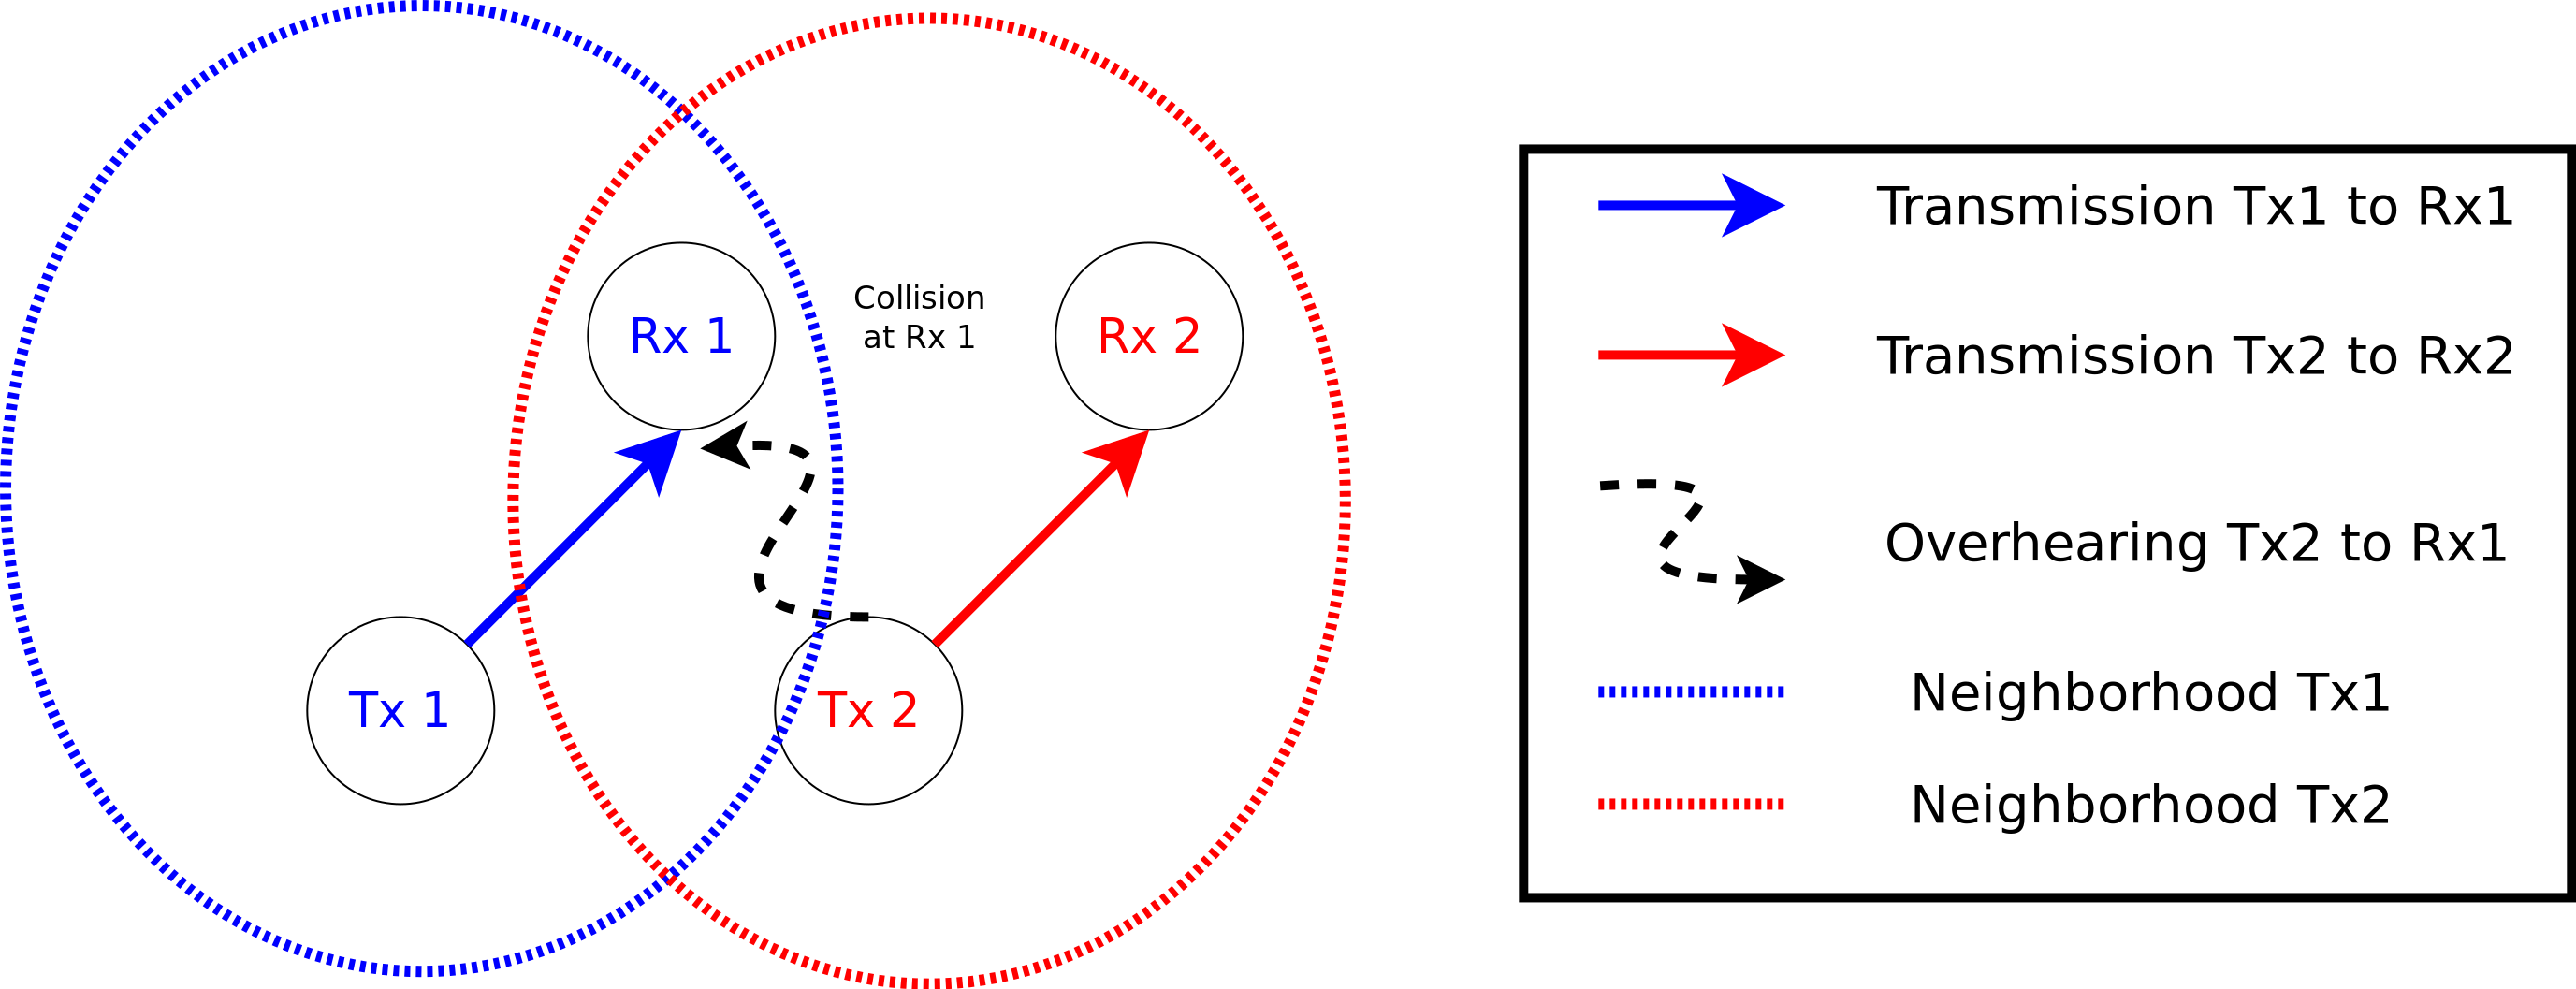
\includegraphics[width=0.8\linewidth]{collision.png}
\end{figure}


\end{frame}
\end{withoutheadline}
%%%%%%%%%%%%%%%%%%%%%%%PROPOSED MECHANISM%%%%%%%%%%%%%%

\section{Proposed Mechanism}

\subsection{Criteria}
\begin{withoutheadline}
\begin{frame}{Proposed Mechanism Criteria}
\begin{itemize}
    \item Our objective is to Reduce the collisions in the dedicated cells.\pause
    \item Using local mutual exclusion we can prevent collisions.\pause  
    \item Since we are working with distributed system, then all the information is local for each node. \pause
    \item Using the 6top transaction we can collect information about neighbors. \pause
    \item From the collected information we can prevent the nodes selecting the same cell. \pause
    \end{itemize}

\end{frame}
\end{withoutheadline}
\subsection{Using 6top Transactions Collect neighbor's cells}
\begin{withoutheadline}
\begin{frame}{Using 6top Transactions Collect neighbor's cells}


\setbeamercolor{block title}{bg=blue!30,fg=black}
\setbeamercolor{block body}{bg=blue!10,fg=black}
\setbeamertemplate{blocks}[rounded][shadow=false]


\begin{block}

    \begin{itemize}
    \item D will transmit an Add request to B.
    \item<2-> B will reply with the Add Response that will contain the cells. 
    \item<3-> The Add Response is transmitted in the shared cell, E \& F will receive and extract the cells.  
    
    \end{itemize}
    \end{block}

\centering

\begin{center}
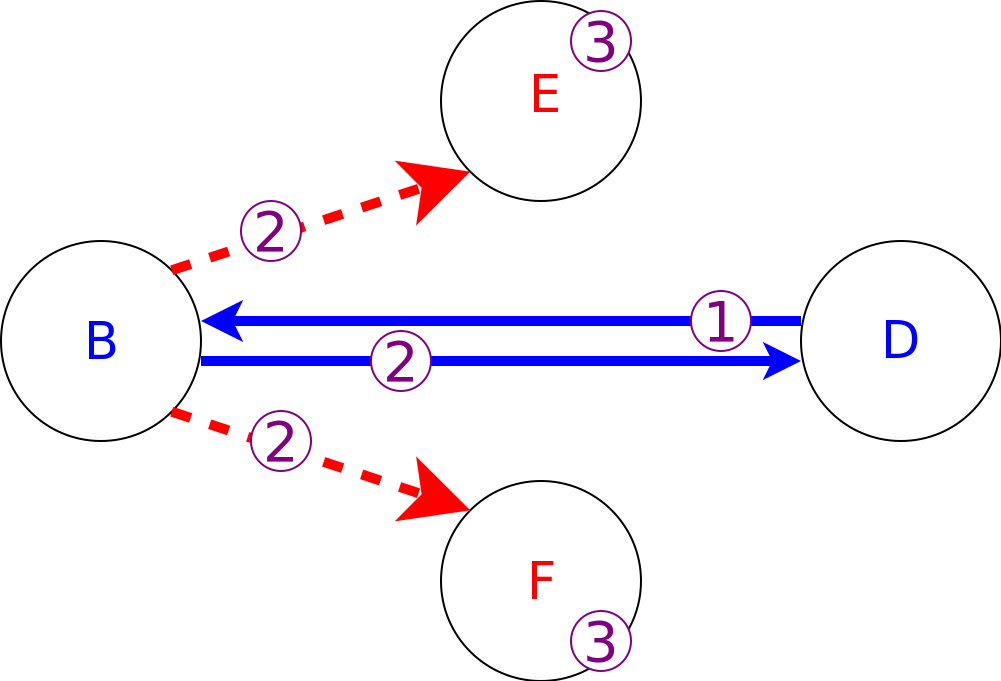
\includegraphics[width=0.6\linewidth]{using6top.png}

\end{center}

\end{frame}
\end{withoutheadline}
\subsection{Avoid Table}
\begin{withoutheadline}
\begin{frame}{Avoid Table}


\setbeamercolor{block title}{bg=blue!30,fg=black}
\setbeamercolor{block body}{bg=blue!10,fg=black}
\setbeamertemplate{blocks}[rounded][shadow=false]


\begin{block}

    \begin{itemize}

    \item The cells reserved by neighbors will be saved by a structure similar to TSCH table. 
    \item<2-> Scheduling function will avoid selecting cells found in this structure. 
    \item<3-> 6top will manage this table.
    \end{itemize}
    \end{block}

\centering
\begin{itemize}
\item[]
\begin{center}
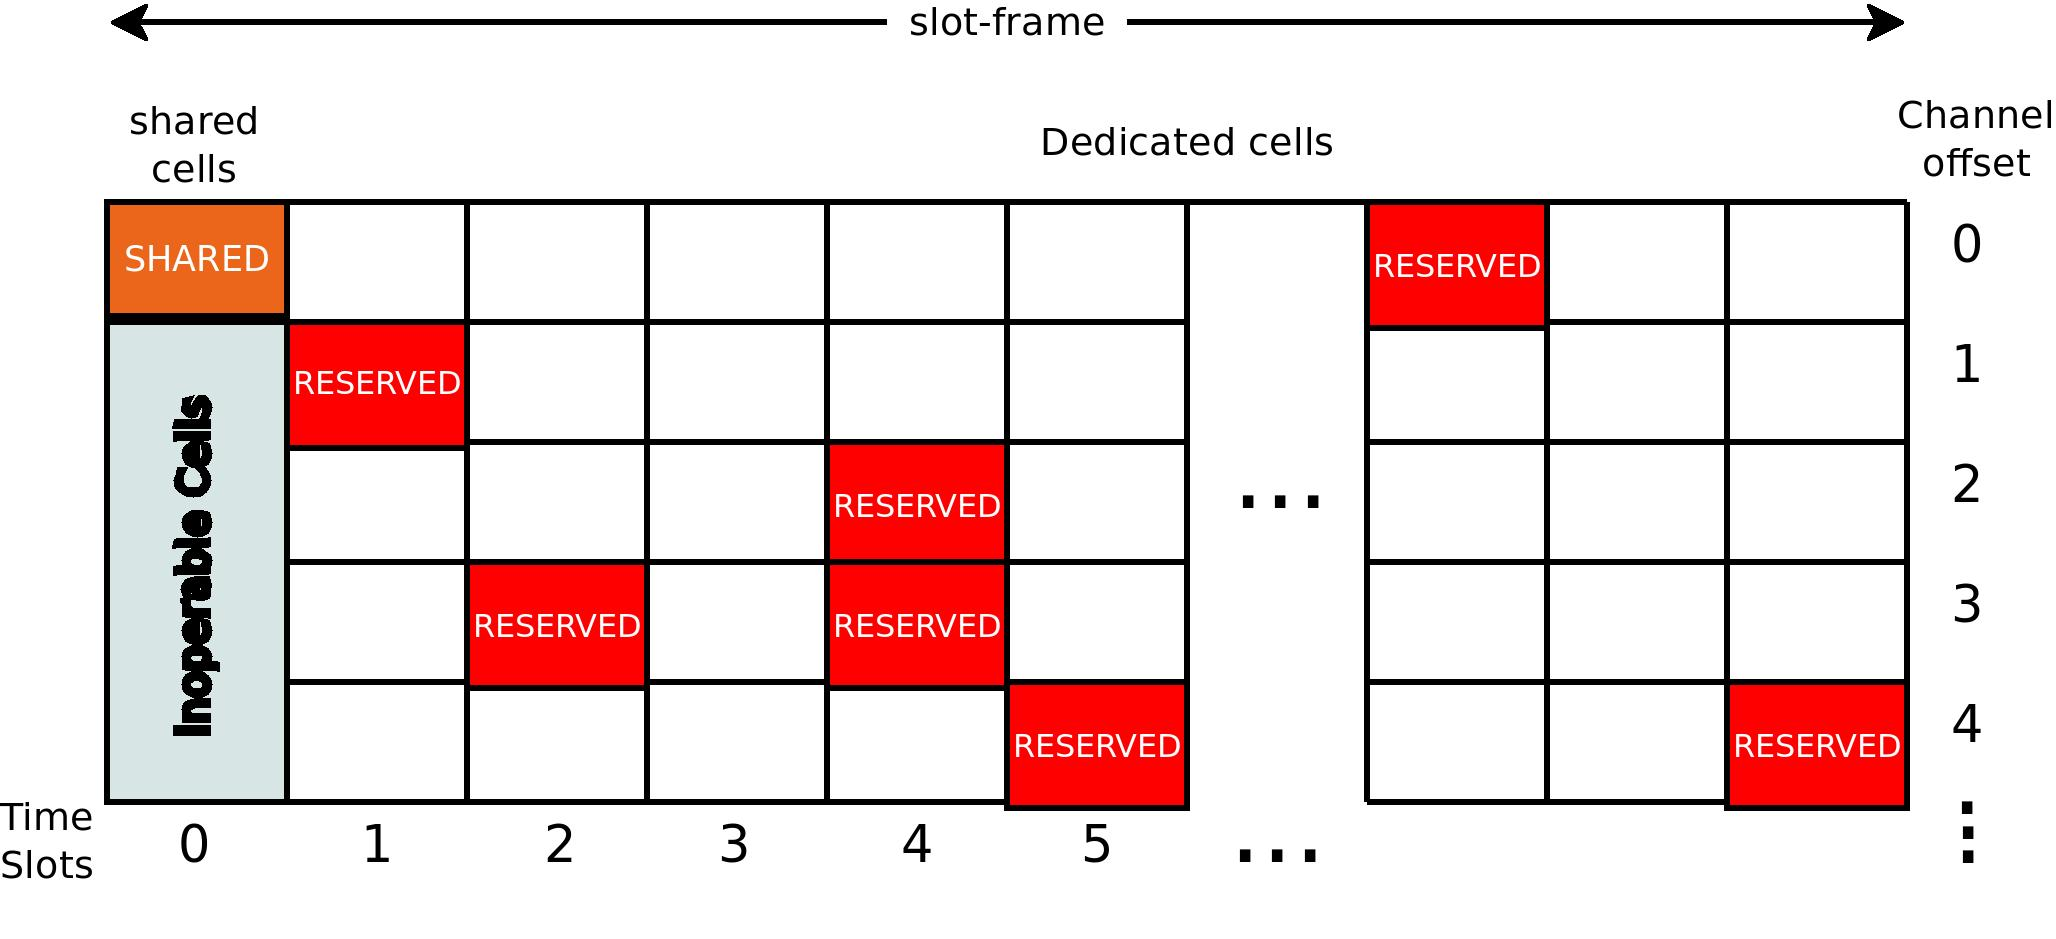
\includegraphics[width=0.8\linewidth]{avoid.jpeg}

\end{center}
\end{itemize}




\end{frame}
\end{withoutheadline}

\subsection{Adding the Cell Buffer}

\begin{withoutheadline}
\begin{frame}{Cell Buffer}


\setbeamercolor{block title}{bg=blue!30,fg=black}
\setbeamercolor{block body}{bg=blue!10,fg=black}
\setbeamertemplate{blocks}[rounded][shadow=false]


\begin{block}

    \begin{itemize}
    \item The assumption of 100\% successful dilevery is not realistic.
    \item<2-> The 6top Transaction maybe lost due too environment effects. 
    \item<3-> The loss of the transaction increase the probability of collisions. 
    \item<4-> By saving the reserved cells in a buffer, and sending the buffer this probability can be reduced.
     
    
    \end{itemize}
    \end{block}

\centering
\begin{figure}[p]

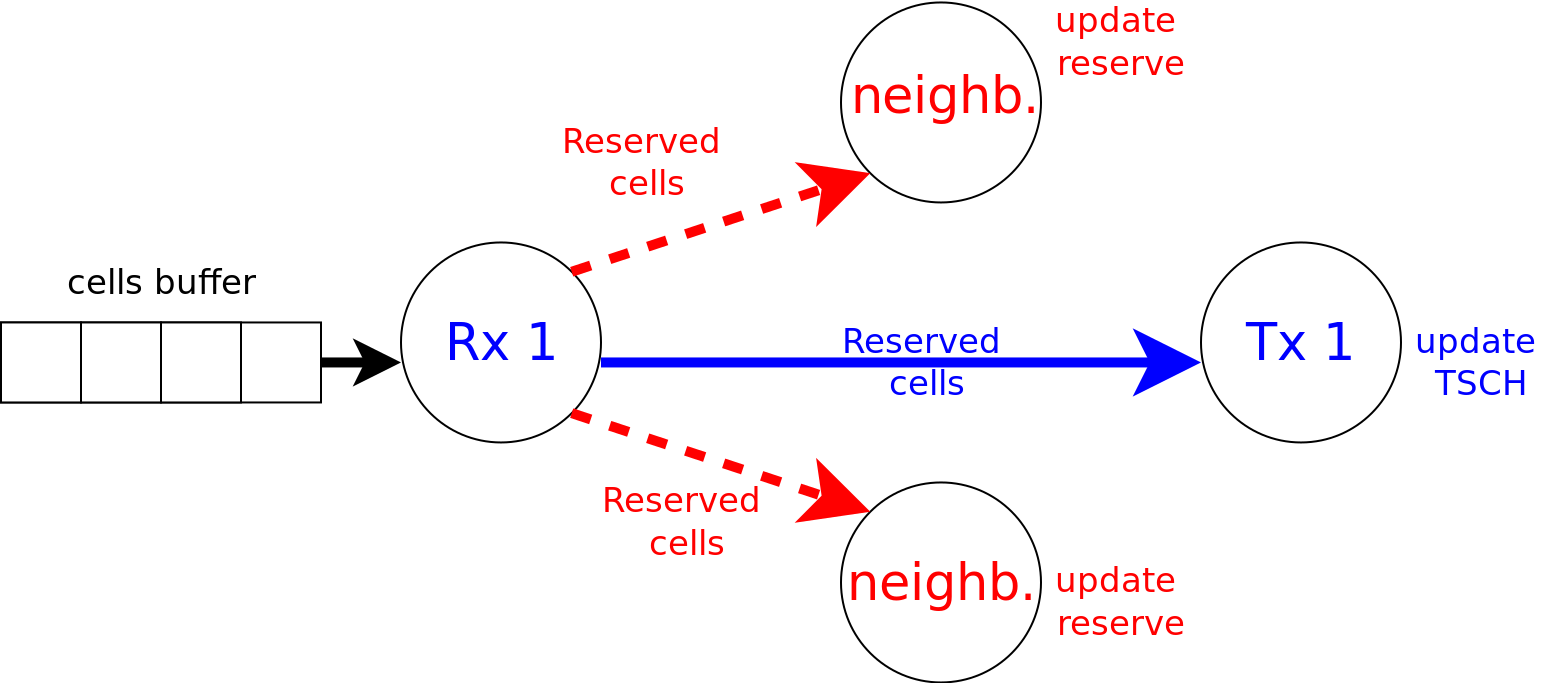
\includegraphics[width=0.7\linewidth]{reserve2.png}
\end{figure}

\end{frame}
\end{withoutheadline}


\begin{withoutheadline}
\begin{frame}{Cell Buffer}

\begin{itemize}
    \item We have created a probablistic model to calaculate the optimal length of the buffer.
    \item<2-> $p$ is the probability of successful transmission.
    \item<3-> we are confidence with a probability $P_{o}$ that one of the transmission is successful.
    \item<4-> $k$ is the number of retransmission (the optimal length of the buffer). 
    \item<5-> we end up with the following equation using binomial distribution:
    
    \end{itemize}
    
 \centering
\begin{figure}[p]

\item<5-> 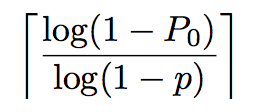
\includegraphics[width=0.3\linewidth]{9nq6n.png}
\end{figure}
\begin{itemize}
\item<6-> According to this equation, and by taking the worst case scenario a buffer of length 10 can assure us 95\% of success
 \end{itemize}
\end{frame}
\end{withoutheadline}
%%%%%%%%%%%%%%%%%%%%%%%RESULTS%%%%%%%%%%%%%%

\section{Simulator and Results}
\subsection{Simulator}
\begin{withoutheadline}
\begin{frame}{Simulator Architecture}


\setbeamercolor{block title}{bg=blue!30,fg=black}
\setbeamercolor{block body}{bg=blue!10,fg=black}
\setbeamertemplate{blocks}[rounded][shadow=false]

\begin{figure}[p]

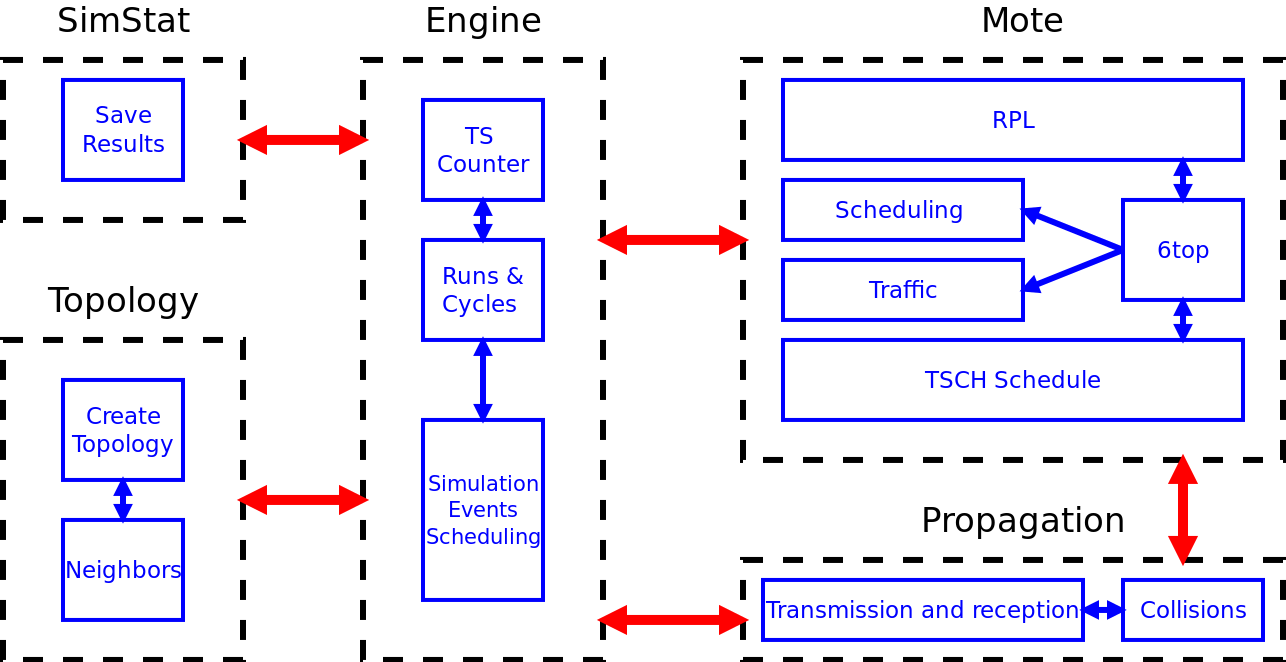
\includegraphics[width=0.95\linewidth]{SIM.png}
\caption{Simulator Architecture}
\end{figure}



\end{frame}
\end{withoutheadline}
\subsection{ Results}
\begin{withoutheadline}
\begin{frame}{Results}

\begin{figure}[p]

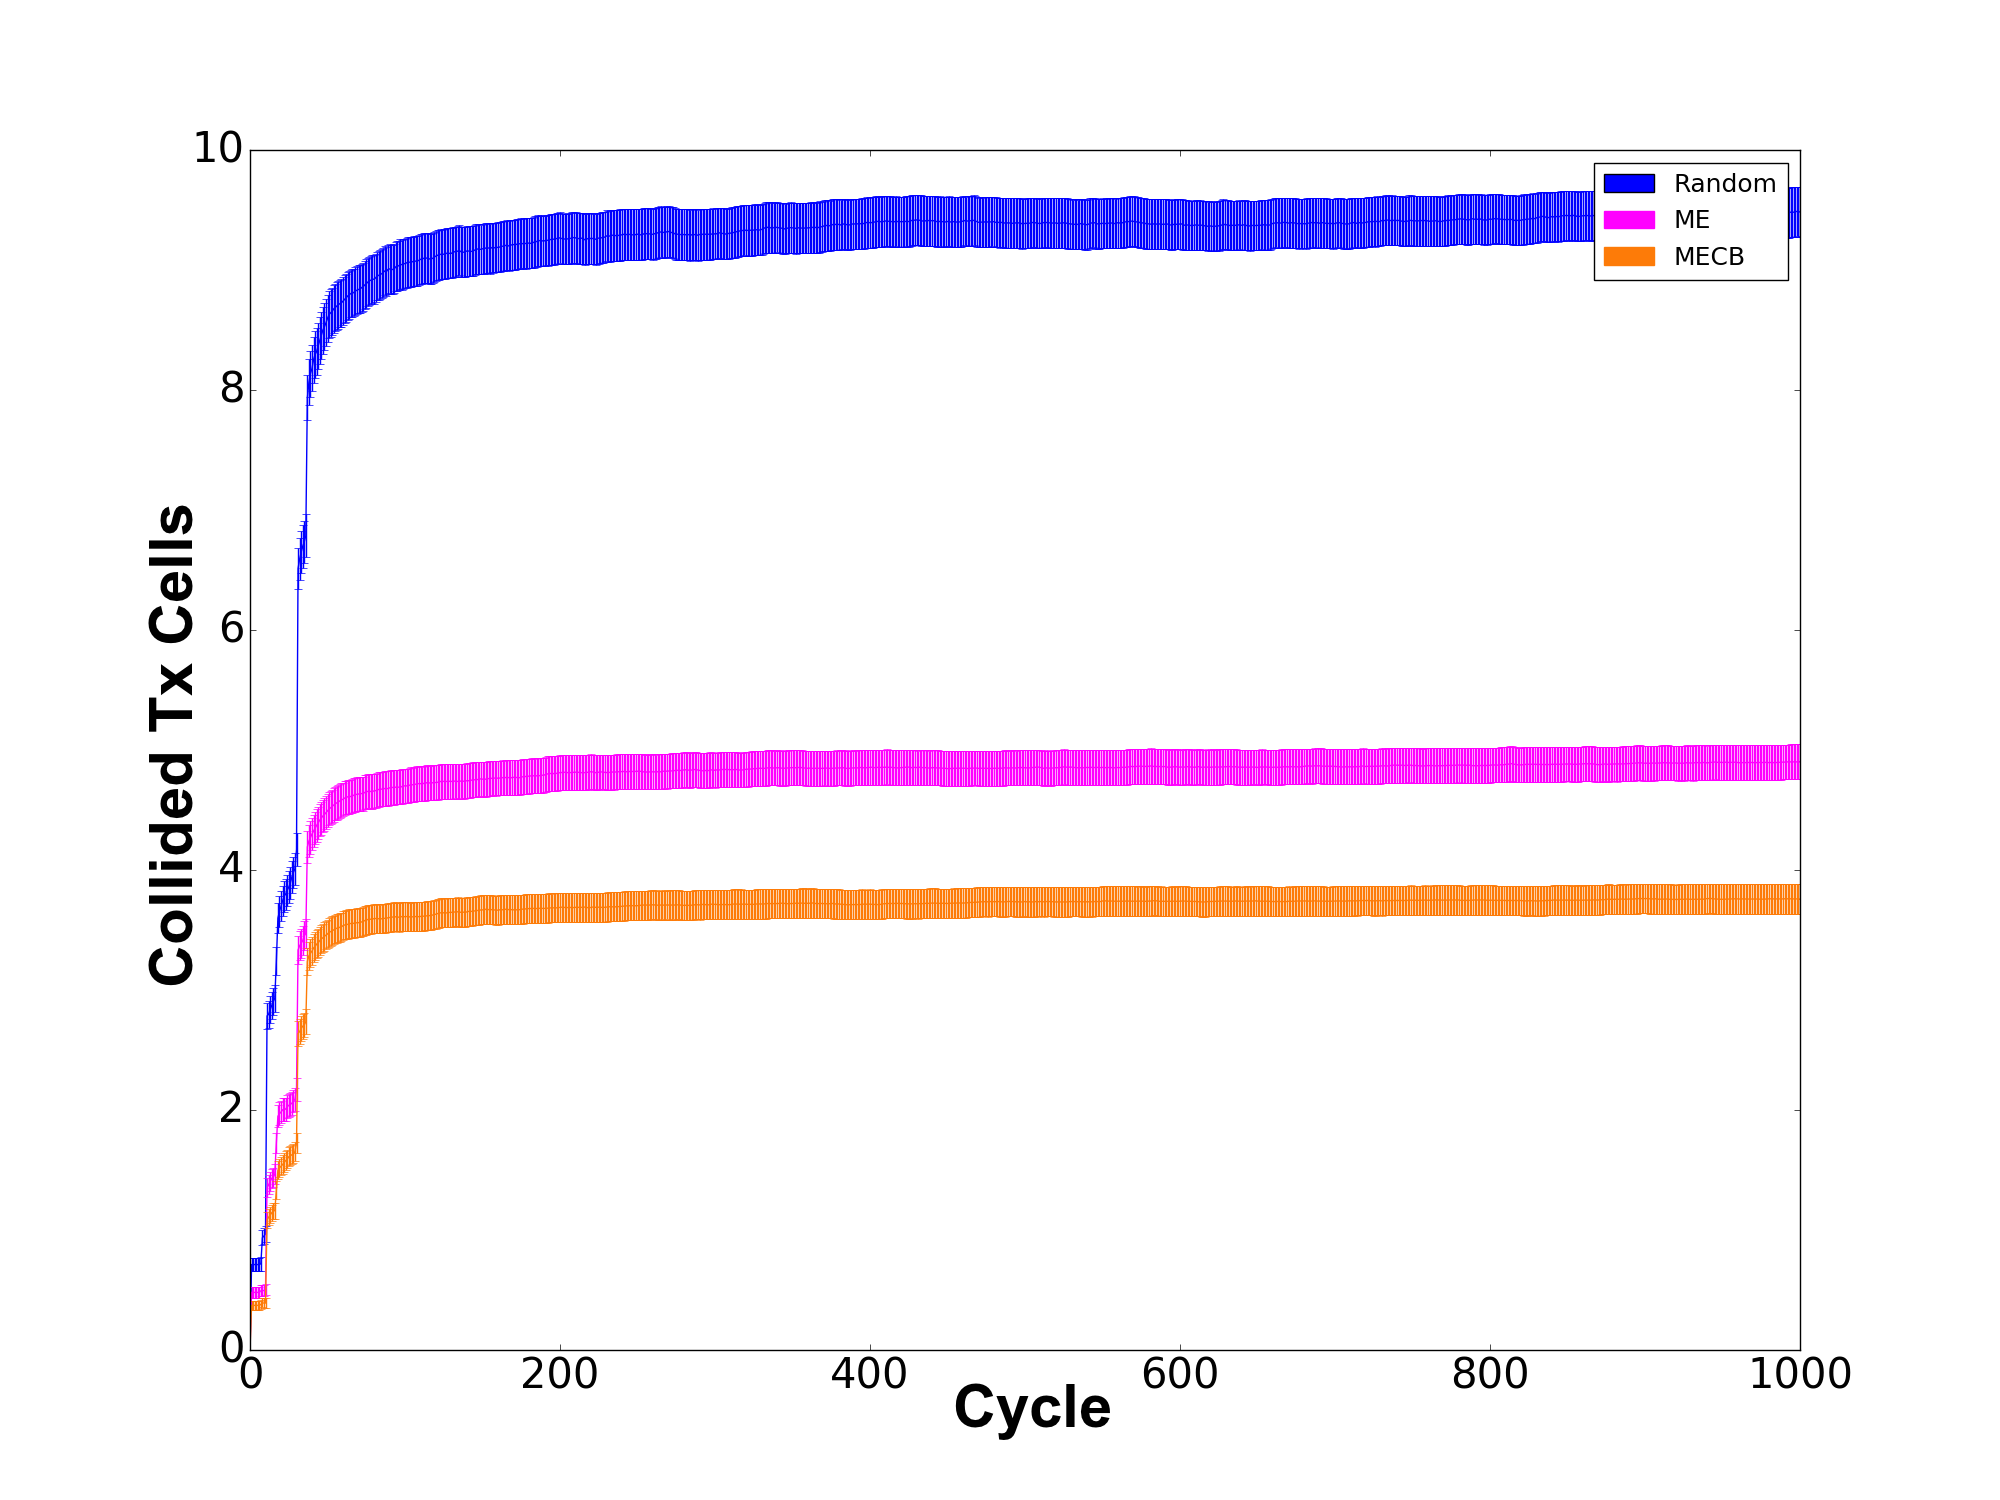
\includegraphics[width=0.8\linewidth]{Graph2.png}
\caption{Simulation of the Number of Collided Tx Cells as Function of Cycle Number (Time)}
\end{figure}



\end{frame}
\end{withoutheadline}




\begin{withoutheadline}
\begin{frame}{Cell Buffer}


\setbeamercolor{block title}{bg=blue!30,fg=black}
\setbeamercolor{block body}{bg=blue!10,fg=black}
\setbeamertemplate{blocks}[rounded][shadow=false]


\begin{block}

    \begin{itemize}
    \item The lost 6top transactions. 
\item<2-> Special Case That Induce Collisions.
    
     
    
    \end{itemize}
    \end{block}

\centering
\begin{figure}[p]

\item<2-> 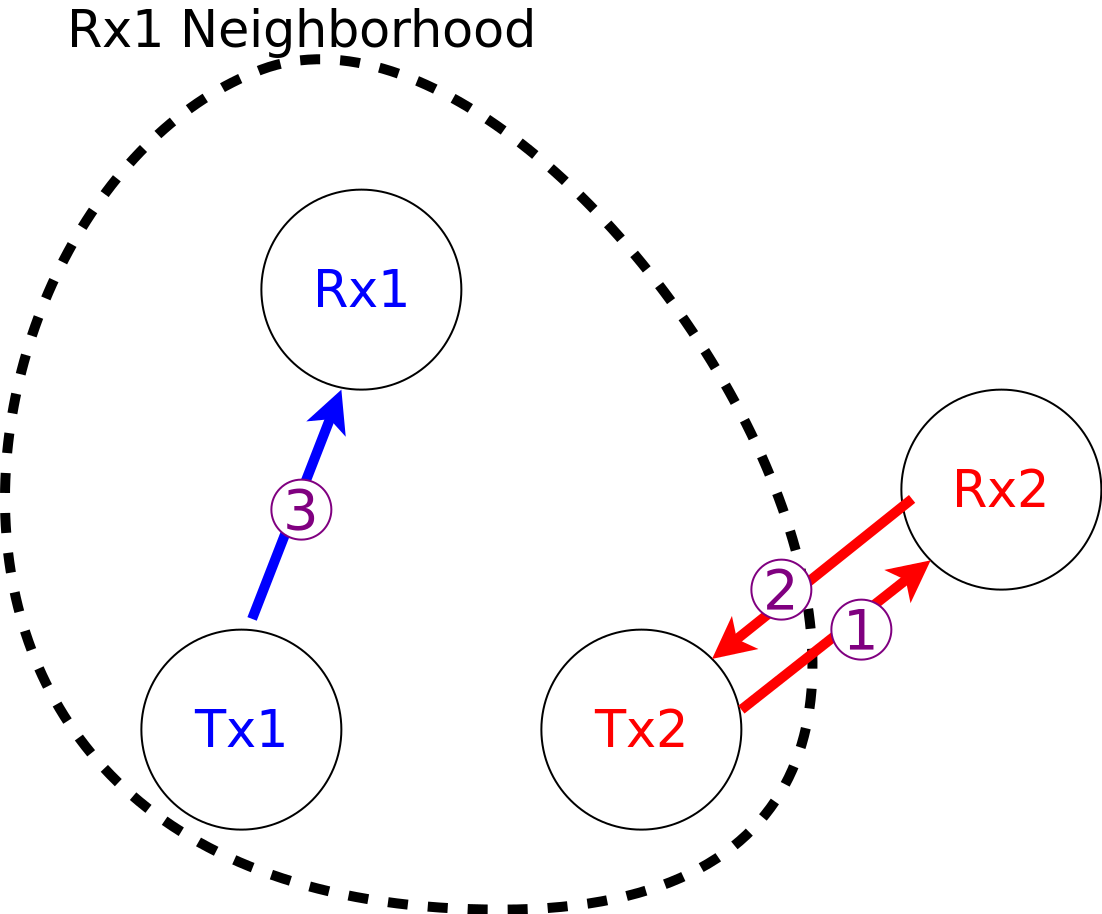
\includegraphics[width=0.4\linewidth]{pro.png}
\end{figure}

\end{frame}
\end{withoutheadline}



\begin{withoutheadline}
\begin{frame}{Comparison with Housekeeping }

\begin{figure}[p]

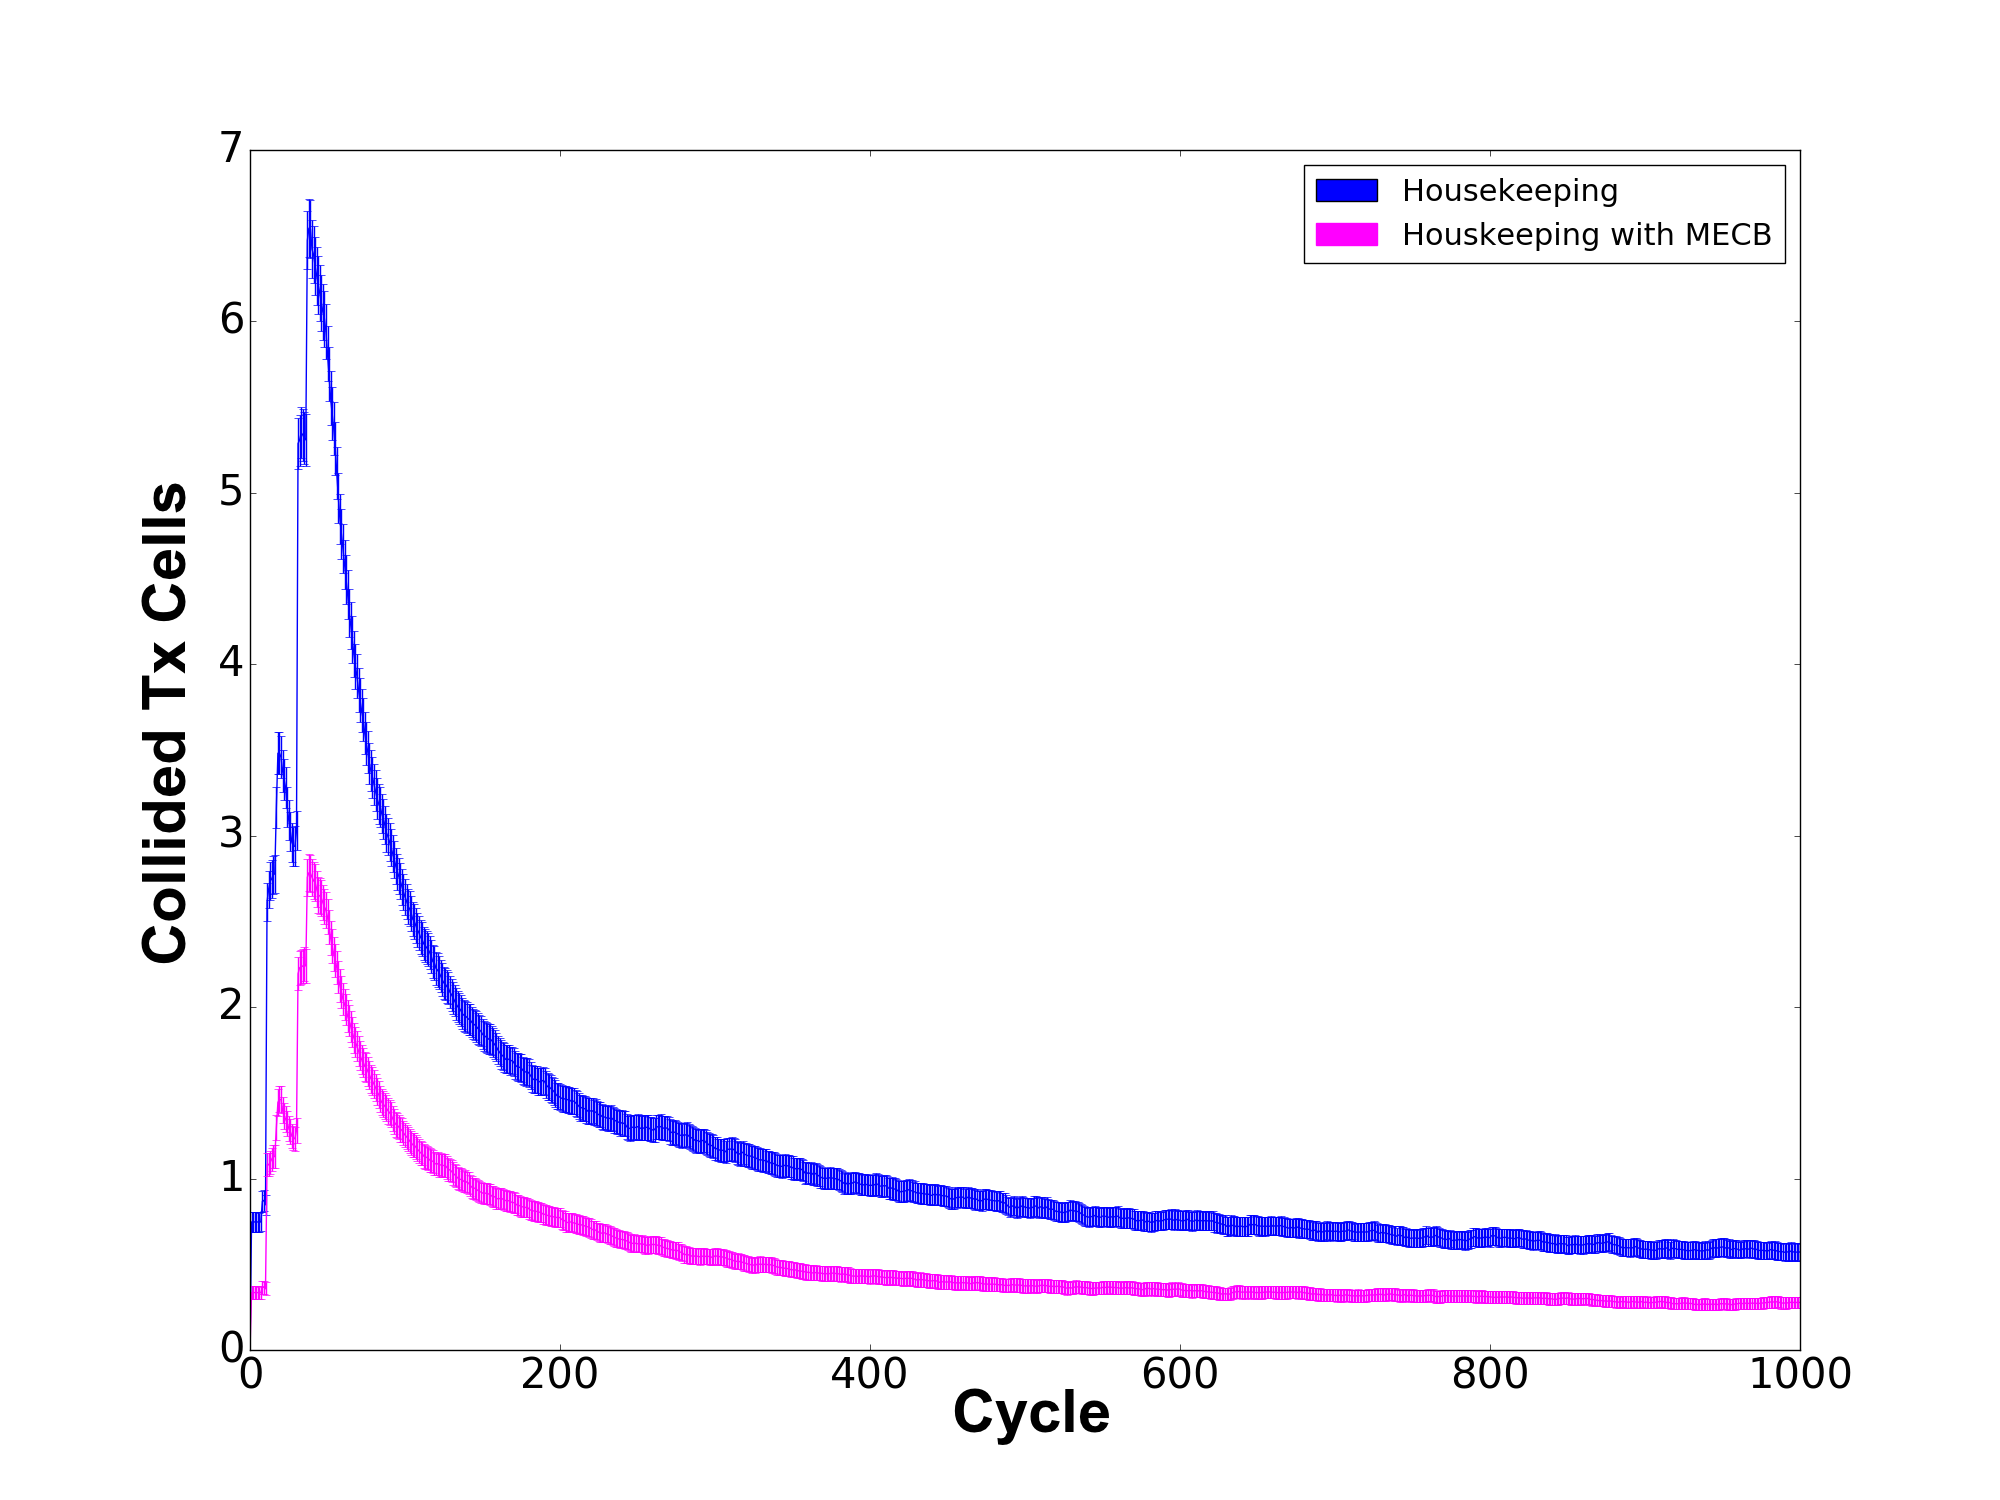
\includegraphics[width=0.8\linewidth]{Graph3.png}
\caption{Simulation of the Number of Collided Tx Cells as Function of Cycle Number (Time) - comparison with the housekeeping approach}
\end{figure}



\end{frame}
\end{withoutheadline}

\begin{withoutheadline}
\begin{frame}{Comparison with Housekeeping}

\begin{figure}[p]

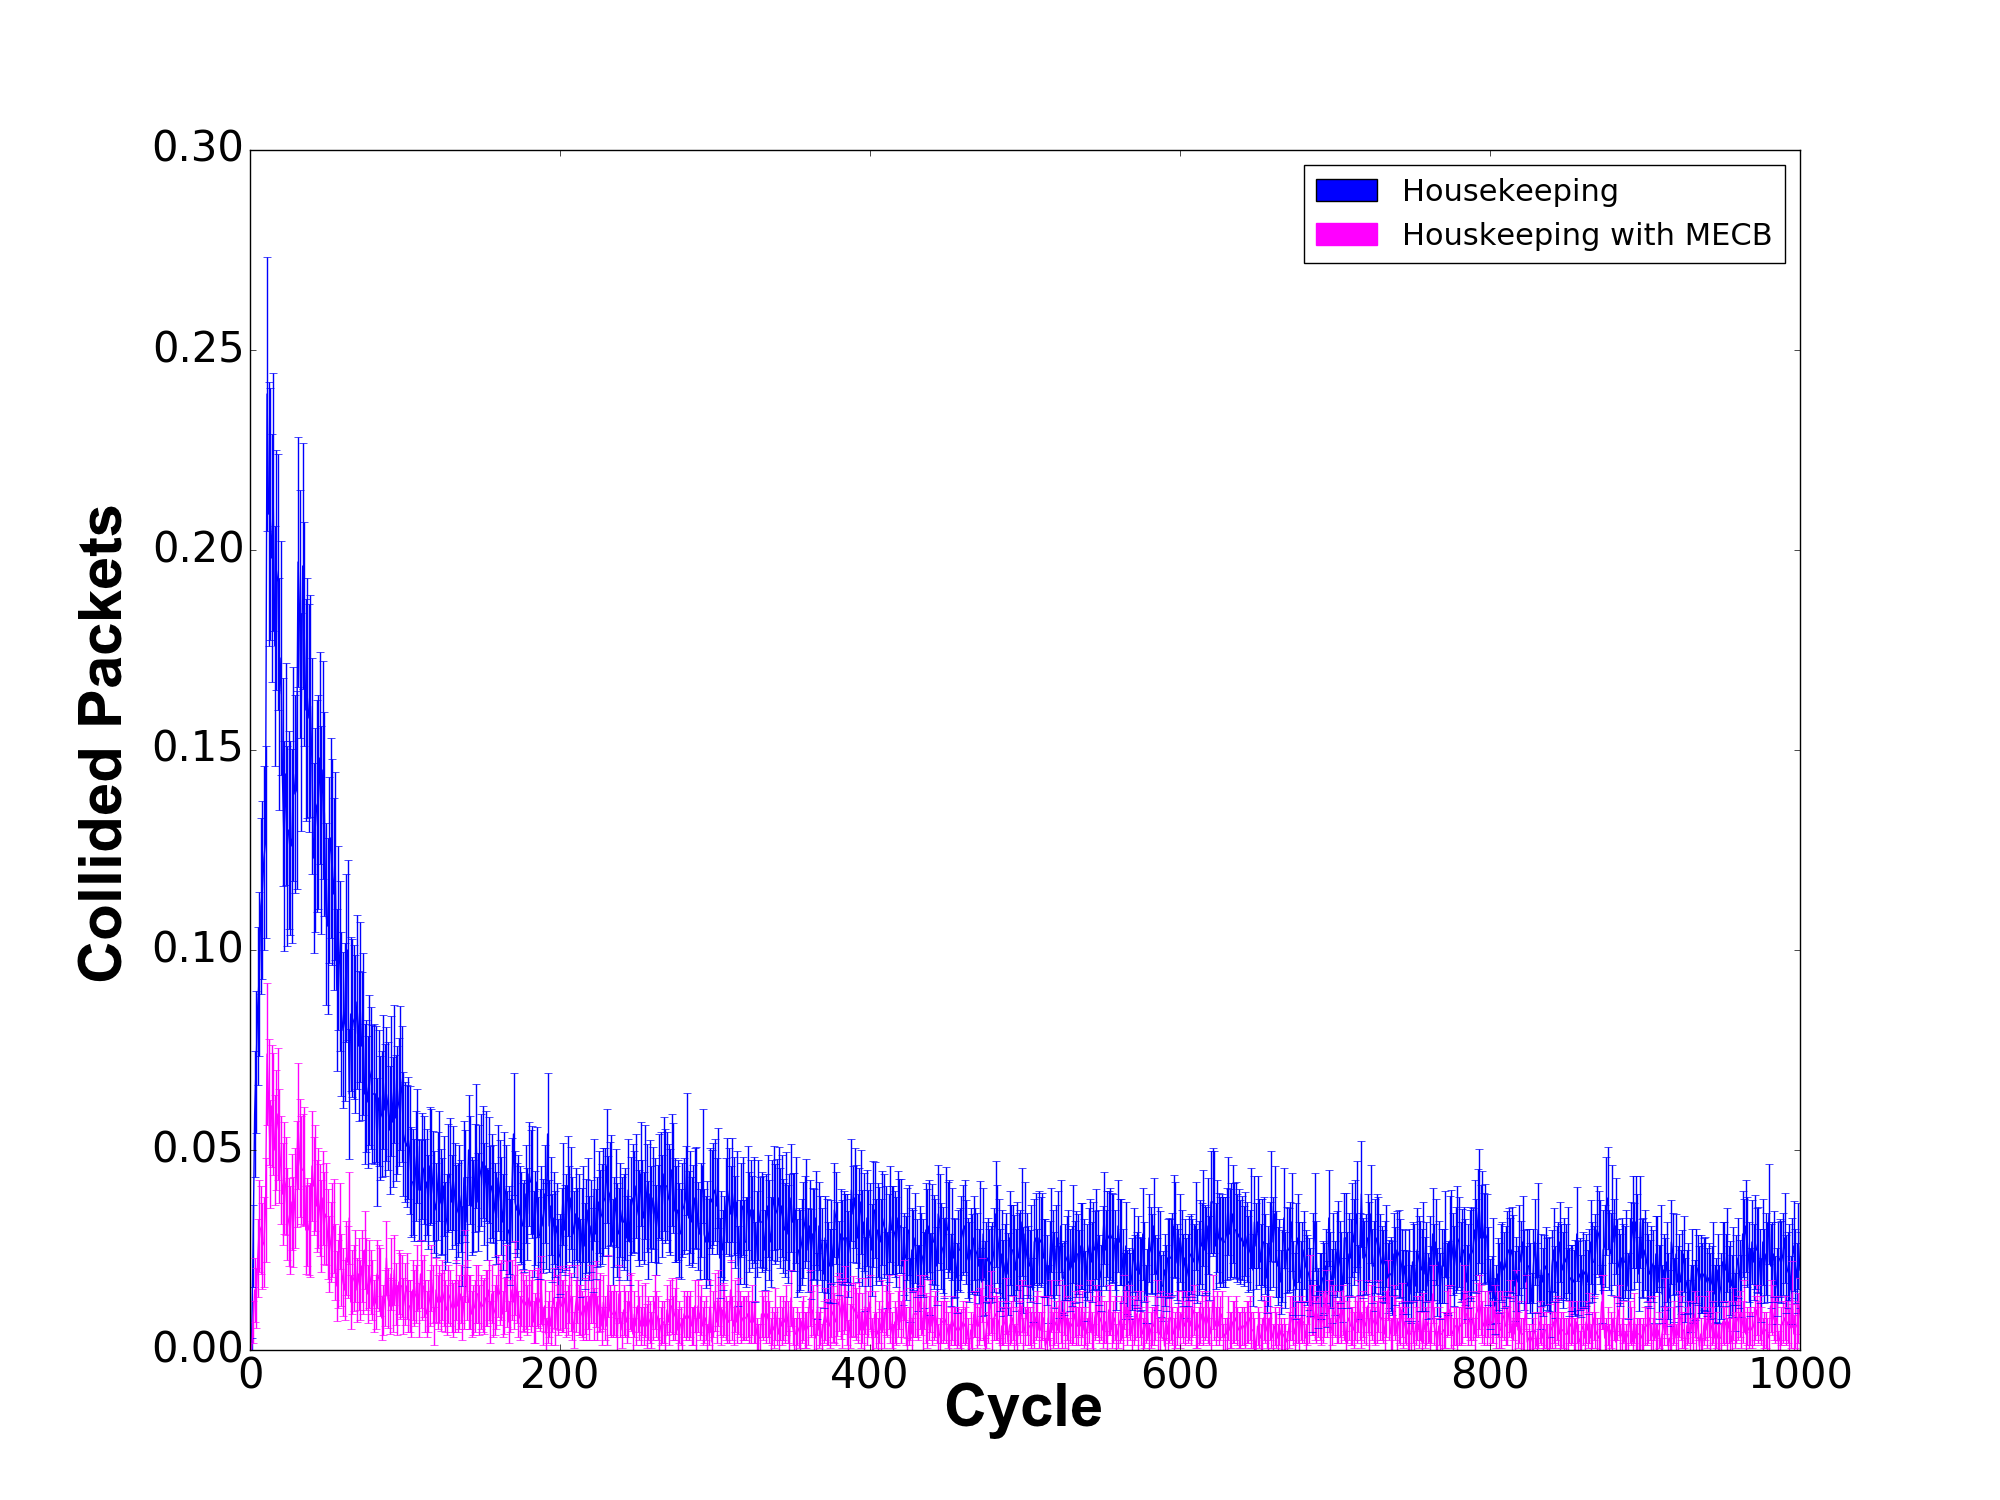
\includegraphics[width=0.8\linewidth]{Graph4.png}
\caption{Simulation of the Number of Collided Packets as Function of Cycle Number (Time) - comparison with the housekeeping approach }
\end{figure}



\end{frame}
\end{withoutheadline}

%%%%%%%%%%%%%%%%%%%%%%%SUMMARY%%%%%%%%%%%%%%
\section*{Summary}
\begin{withoutheadline}
\begin{frame}{Summary}
  \begin{itemize}
  \item
    Our implementation introduce  \alert{no overhead } in the network.
  \item
    The implementation \alert{achieved 60\% reduction} in the number of collided Tx cells and \alert{70\% reduction} of the Collided Packets.
  \item The Combination of Our approach and Housekeeping accomplish an \alert{ almost collision free dedicated cells}.
  \end{itemize}
  
  \begin{itemize}
  \item
    Outlook
    \begin{itemize}
    \item
     Our goal is to reach a place were we have collision free network, using more complex methods.
    \item
      Our prespective in this project was work on 6top, but our next steps is to study the effects of traffic in the protocols performances.
    \end{itemize}
  \end{itemize}
\end{frame}
\end{withoutheadline}

\section*{last}


\begin{withoutheadline}
\begin{frame}


\setbeamercolor{block title}{bg=blue!30,fg=black}
\setbeamercolor{block body}{bg=blue!10,fg=black}
\setbeamertemplate{blocks}[rounded][shadow=false]
\begin{tabular}{ccc}

\includegraphics[page=15, width=0.3\textwidth]{ali.pdf} &

\includegraphics[page=19, width=0.3\textwidth]{ali.pdf} &

\includegraphics[page=43, width=0.3\textwidth]{ali.pdf} \\


\includegraphics[page=54, width=0.3\textwidth]{ali.pdf} &

\includegraphics[page=66, width=0.3\textwidth]{ali.pdf} &

\includegraphics[page=69, width=0.3\textwidth]{ali.pdf} \\




\end{tabular}

\begin{block}{}
\centering Thanks for your attention!\\
Questions?
\end{block}
\end{frame}
\end{withoutheadline}
\end{document}


